% IF YOU ARE USING OVERLEAF, MAKE SURE TO SET THE COMPILER TO XeLatex.

\documentclass[final]{beamer}

% ====================
% Packages
% ====================

\usepackage[T1]{fontenc}
\usepackage{lmodern}
\usepackage[size=custom,width=91.44,height=60.96,scale=0.83]{beamerposter}
\usetheme{gemini}
\usecolortheme{stanford}
\usepackage{graphicx}
\usepackage{booktabs}
\usepackage{tikz}
\usetikzlibrary{shapes,arrows,positioning,calc}
\usepackage{pgfplots}
\usepackage{amsmath}
\usepackage{amssymb}
\usepackage{siunitx}
\pgfplotsset{compat=1.17}
\graphicspath{{figures/project/}{stanford_logos/}}

% Tighten vertical spacing between poster blocks.
\addtobeamertemplate{block end}{}{\vspace{-0.45cm}}

% ====================
% Lengths
% ====================

\newlength{\sepwidth}
\newlength{\colwidth}
\setlength{\sepwidth}{0.01\paperwidth}
\setlength{\colwidth}{0.32\paperwidth}
\newcommand{\separatorcolumn}{\begin{column}{\sepwidth}\end{column}}

% ====================
% Title
% ====================

\title{Decision Transformer Warm-Start for Minimum-Time Vehicle Trajectory Optimization}
\author{Sebastian Martinez}
\institute[shortinst]{Department of Aeronautics \& Astronautics, Stanford University}

\footercontent{
  \href{mailto:sebasmp@stanford.edu}{sebasmp@stanford.edu} \hfill
  Stanford CS234: Reinforcement Learning \hfill
  Decision Transformer Warm-Starts for Trajectory Optimization
}

\begin{document}

\addtobeamertemplate{headline}{}
{
    \begin{tikzpicture}[remember picture,overlay]
      \node [anchor=north east, inner sep=3cm] at ([xshift=1.0cm,yshift=2.5cm]current page.north east)
      {
\includegraphics[height=6.0cm]{Block_S_2_color.png}};
    \end{tikzpicture}
}

\begin{frame}[t]
\begin{columns}[t]
\separatorcolumn

\begin{column}{\colwidth}

\begin{block}{Problem}
Minimum-time racing line optimization is a drive-at-the-limits planning problem in which lateral and longitudinal forces must be coordinated near the tire friction boundary while satisfying strict track and safety constraints. In this regime, solver performance depends strongly on model fidelity and initialization quality: small changes in the initial guess can change convergence speed, local optimality, and even feasibility \cite{aggarwal2025friction}.

The project studies whether an offline sequence model can amortize this nonlinear constrained optimization problem by supplying a better warm start. The target setting is closed-track autonomous racing with nonlinear vehicle dynamics, hard track boundaries, and static obstacle-avoidance constraints.

The system is two-stage: a production optimizer based on spatial direct collocation and a single-track vehicle model generates expert trajectories, while a Decision Transformer (DT) learns from this offline data to predict warm-start trajectories $(X_{\text{init}}, U_{\text{init}})$. The goal is to reduce solver iterations and wall-clock solve time without sacrificing feasibility or lap time quality.

This hybrid framing keeps hard dynamics and safety constraints inside the optimizer while shifting part of the repeated search effort into an offline-trained sequence model.
\end{block}

\begin{block}{Background}
The production planner solves a \textbf{minimum-time NLP} in Frenet/arc-length coordinates using \textbf{spatial direct collocation}. The decision variables are the state and control values at $N{+}1$ spatial nodes, and the dynamics are enforced with trapezoidal integration in spatial form.

\textit{State:} $x = [u_x,\;u_y,\;r,\;\Delta F_{z,\ell},\;\Delta F_{z,\mathrm{lat}},\;t,\;e,\;\Delta\psi]^\top \in \mathbb{R}^{8}$

\textit{Control:} $u = [\delta,\;F_x]^\top \in \mathbb{R}^{2}$
\begin{align*}
 \min_{x_{0:N},\,u_{0:N}} \quad & t_N \;+\; \lambda_u\sum_{k=0}^{N-1}\lVert u_{k+1}-u_k\rVert^2 \\[4pt]
\text{s.t.} \quad
& x_{k+1} = x_k + \frac{\Delta s}{2}\Big(f_s(x_k,u_k)+f_s(x_{k+1},u_{k+1})\Big), \quad k=0,\dots,N-1 \\
& e_{\min}(s_k)\le e_k\le e_{\max}(s_k),\quad |\delta_k|\le\delta_{\max},\quad F_{x,\min}\le F_{x,k}\le F_{x,\max} \\
& \dot{s}_k \ge \epsilon_s,\quad 1-\kappa(s_k)e_k \ge \epsilon_\kappa \\
& \lVert p(s_k,e_k)-p_{\mathrm{obs},i}\rVert^2 \ge R_{\mathrm{safe},i}^2 \quad \forall\,i,\,k \\
& t_0 = 0,\quad x_0 = x_N,\quad u_0 = u_N \quad \text{(full lap with periodic closure except time)}
\end{align*}

$R_{\mathrm{safe},i} = r_i + \mathrm{margin}_i + R_{\mathrm{vehicle}}$. Obstacle constraints are enforced at nodes and interior samples, then checked again with dense post-solve collision validation and acceptance-gated retries.
\end{block}

\begin{block}{Background: Decision Transformer}
Decision Transformer casts offline reinforcement learning as conditional sequence modeling over expert trajectories \cite{chen2021decision}. Instead of learning a value function or policy through online interaction, the model is trained on optimizer-generated trajectories and conditions on return-to-go, past observations, and past actions. Here, the return-to-go is derived from minimum-time cost, so higher return corresponds to lower remaining lap time.

The DT is not used as the final controller. It is used to propose a dynamically coherent trajectory that is good enough to reduce downstream solver work. Compared with standalone policy execution, this keeps hard constraints and high-fidelity vehicle dynamics inside the optimization layer. The setup is therefore closer to learned warm-starting for trajectory optimization than to end-to-end policy replacement \cite{guffanti2024transformers}.
\end{block}

\end{column}

\separatorcolumn

\begin{column}{\colwidth}

\begin{block}{Methods}
\begin{center}
\begin{tikzpicture}[
    node distance=2.3cm,
    box/.style={rectangle, draw, rounded corners, minimum height=1.0cm, text width=3cm, align=center, font=\small},
    arrow/.style={->, >=stealth, thick}
]
\node[box, fill=blue!18] (data) {Accepted Expert\\Trajectories};
\node[box, fill=green!18, right=of data] (dt) {Decision\\Transformer};
\node[box, fill=orange!18, right=of dt] (ws) {Warm-Start\\Rollout};
\node[box, fill=red!15, right=of ws] (nlp) {FATROP / IPOPT\\NLP};
\node[box, fill=gray!18, right=of nlp] (sol) {Feasible Minimum-Time\\Trajectory};

\draw[arrow] (data) -- node[above, font=\scriptsize, align=center] {offline\\training} (dt);
\draw[arrow] (dt) -- node[above, font=\scriptsize] {$X_{\mathrm{init}},U_{\mathrm{init}}$} (ws);
\draw[arrow] (ws) -- node[above, font=\scriptsize, align=center]
{accept or\\fallback} (nlp);
\draw[arrow] (nlp) -- node[above, font=\scriptsize] {refinement} (sol);
\end{tikzpicture}
\end{center}

\begin{center}
\scriptsize\textit{Figure 1. Offline warm-start pipeline.}
\end{center}

\vspace{0.4em}

\begin{center}
\begin{tikzpicture}[
    node distance=0.5cm,
    tok/.style={rectangle, draw, rounded corners, minimum height=0.8cm, text width=1.55cm, align=center, font=\scriptsize},
    proc/.style={rectangle, draw, rounded corners, minimum height=0.95cm, text width=2.45cm, align=center, font=\scriptsize},
    arrow/.style={->, >=stealth, thick}
]
\node[tok, fill=blue!14] (rtgk) {$R_k$};
\node[tok, fill=blue!14, right=of rtgk] (xk) {$\tilde{x}_k$};
\node[tok, fill=blue!14, right=of xk] (uk) {$u_k$};
\node[tok, fill=blue!14, right=of uk] (rtgkp) {$R_{k+1}$};
\node[tok, fill=blue!14, right=of rtgkp] (xkp) {$\tilde{x}_{k+1}$};
\node[tok, fill=blue!14, right=of xkp] (ukp) {$u_{k+1}$};
\node[proc, fill=green!14, right=0.75cm of ukp] (embed) {Embeddings};
\node[proc, fill=orange!18, right=of embed] (trans) {Causal DT\\$K=50$, 6L, 4H, 192D};
\node[proc, fill=gray!18, right=of trans] (head) {Predict $\hat{u}_k$\\and $\hat{x}_{k+1}$};

\draw[arrow] (rtgk) -- (xk);
\draw[arrow] (xk) -- (uk);
\draw[arrow] (uk) -- (rtgkp);
\draw[arrow] (rtgkp) -- (xkp);
\draw[arrow] (xkp) -- (ukp);
\draw[arrow] (ukp) -- (embed);
\draw[arrow] (embed) -- (trans);
\draw[arrow] (trans) -- (head);
\end{tikzpicture}
\end{center}

\begin{center}
\scriptsize\textit{Figure 2. Decision Transformer tokenization and prediction flow.}
\end{center}

The learning problem is framed as \textbf{offline RL via sequence modeling}. Figure 1 shows the overall warm-start pipeline: the nonlinear optimizer generates accepted expert trajectories offline, the Decision Transformer is trained on this dataset, and at test time it autoregressively generates a candidate rollout that is passed to the downstream NLP if it survives the wrapper checks. Figure 2 shows the DT formulation more directly. Each rollout is converted into a token sequence of return-to-go, augmented state, and action, where the augmented state includes the local vehicle/path state $(u_x,u_y,r,e,\Delta\psi)$ together with track geometry and padded obstacle context. Return-to-go is computed from negative time increments, so larger return corresponds to less remaining lap time.

At training time, the DT is fit with a supervised objective consisting of action prediction plus an auxiliary next-state loss,
\[
\mathcal{L} = \mathcal{L}_{a} + \lambda_x \mathcal{L}_{x},
\]
with the latest improved parent run using $\lambda_x=0.1$. The main architecture used in the current improved family has context length $K=50$, $6$ transformer layers, $4$ attention heads, embedding size $192$, batch size $128$, and dropout $0.1$. At inference, the model autoregressively predicts actions, rolls them forward through the vehicle dynamics, and produces a candidate warm-start trajectory for the downstream optimizer.
\end{block}

\begin{block}{Experiments}
Experiments are run in an Oval-first benchmark with two frozen scenario families: a no-obstacle gate and a frozen obstacle gate with 1--4 circular obstacles. The DT is trained on several sources of optimizer-generated data. The largest source is a shift dataset of accepted full-lap solutions circularly shifted along the track, and this is complemented by hard-repair, post-projection repair, and failure-conditioned repair segments that target more difficult rollout states.

The current FATROP-clean Oval dataset contains 31{,}710 shift episodes, 400 hard repairs, 1{,}000 post-projection repairs, and 300 failure-conditioned repairs. The model input consists of return-to-go, local vehicle/path state, track features, and nearest-obstacle context, and the output is a warm-start control sequence together with the rolled-out state trajectory. Evaluation is solver-facing: the main metrics are warm-start acceptance, fallback behavior, solver iterations, and total solve time.
\end{block}

\begin{block}{Experiments: Optimization Output}
\begin{figure}
  \centering
  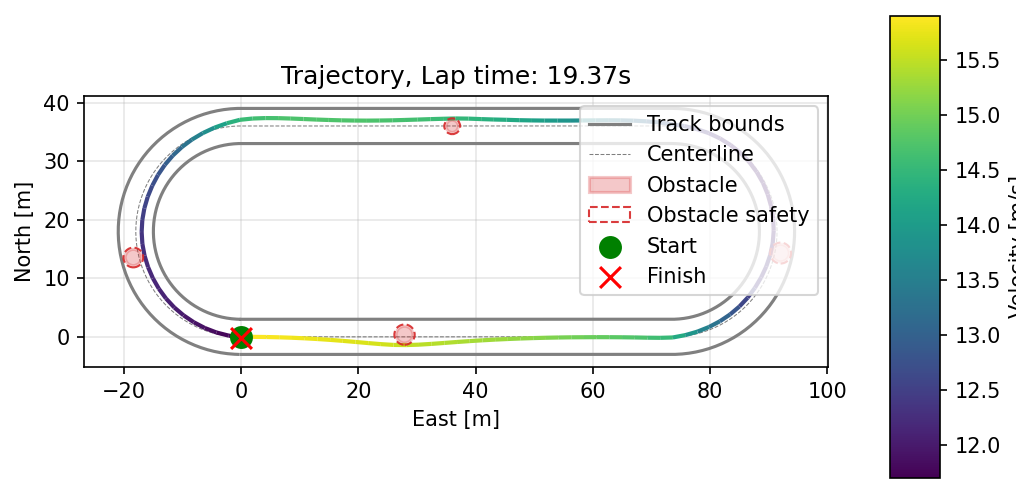
\includegraphics[width=0.88\linewidth]{fatrop_oval_obstacles_traj.png}
  \caption{Representative obstacle-aware trajectory optimization result on the oval track. The production optimizer produces feasible, obstacle-avoiding full-lap solutions that are used as expert data.}
\end{figure}
\end{block}

\begin{block}{Analysis}
\begin{figure}
  \centering
  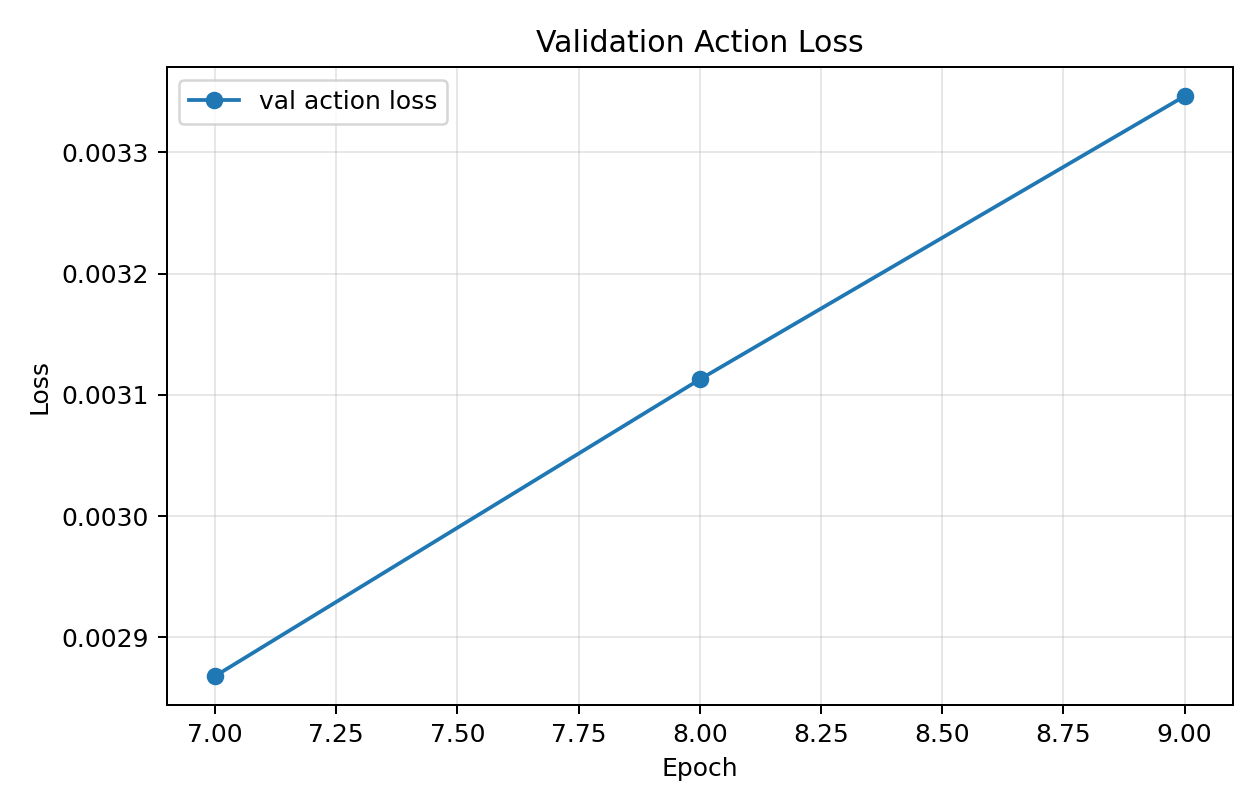
\includegraphics[width=0.47\linewidth]{postproj_ft2_val_loss_curves.png}
  \hfill
  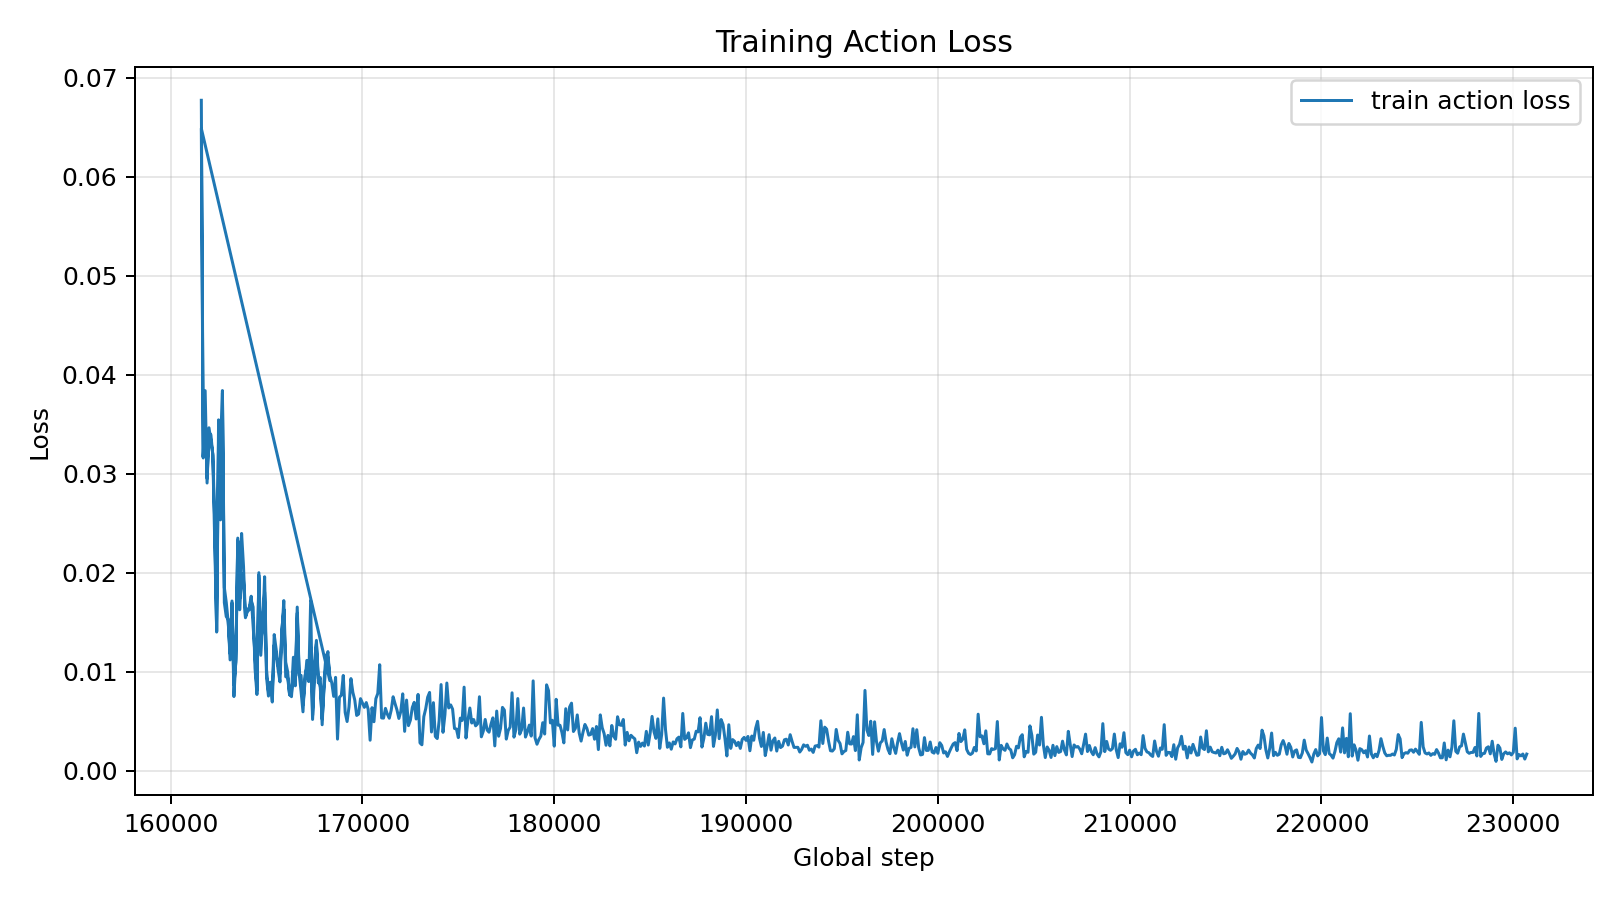
\includegraphics[width=0.47\linewidth]{postproj_ft2_train_loss_curves.png}
  \caption{Validation action loss (left) and training action loss (right) for the post-projection FT2 rerun. The larger-context improved training family produced stable optimization and provided the parent checkpoint used for subsequent fine-tuning experiments.}
\end{figure}
\end{block}

\end{column}

\separatorcolumn

\begin{column}{\colwidth}

\begin{block}{Results and Interpretation}
Best offline results among the current improved checkpoints:
\begin{itemize}
  \item `ctx50\_m6x192`: best val loss `0.002835`, best val action loss `0.002600`
  \item `lateral\_ft`: best val loss `0.002773`, best val action loss `0.002544`
  \item `failure\_ft`: best val loss `0.002364`, best val action loss `0.002197`
\end{itemize}

Latest completed solver-facing comparisons:
\begin{itemize}
  \item under the completed projection ablation, the best DT operating point was `postproj\_ft2\_rerun + projection=soft`
  \item in these completed fixed-gate comparisons, DT solve time was often slightly below baseline
  \item the main deployment metrics remained warm-start acceptance, solver iterations, and total solve time
\end{itemize}

\textbf{Interpretation}
\begin{itemize}
  \item \textbf{Optimization backbone works.} The direct-collocation solver reliably generates accepted obstacle-aware expert trajectories.
  \item \textbf{Offline DT fit improved strongly over older runs.} The larger-context improved family reduced validation losses substantially.
  \item \textbf{Data interventions were implemented beyond nominal imitation.} The pipeline now includes post-projection and failure-conditioned repair data, not only clean shift episodes.
  \item \textbf{Offline ranking and deployment ranking are not identical.} The best offline checkpoint is `failure\_ft`, while the best completed deployment operating point in the projection ablation was `postproj\_ft2\_rerun + soft`.
  \item \textbf{Conclusion:} the project now has a stable data, training, and evaluation pipeline for studying learned warm-starts on nonlinear trajectory optimization.
\end{itemize}
\end{block}

\begin{block}{Conclusions and Next Steps}
\begin{itemize}
  \item A full offline-data pipeline exists for constrained racing trajectory optimization with nonlinear dynamics and obstacle handling.
  \item The improved DT family achieves substantially better offline validation losses than older runs.
  \item The hybrid DT + optimizer architecture is operational, including rollout generation, repair-data production, and warm-start benchmarking.
  \item Completed comparisons identified both a best offline checkpoint and a best deployment operating point for the current Oval-first benchmark regime.
  \item convert the current Oval-first benchmark and diagnosis pipeline into a polished final report and poster-ready artifact set
  \item extend checkpoint comparisons on identical frozen no-obstacle and obstacle scenario sets
  \item continue checkpoint selection using acceptance, iterations, and total solve time rather than offline loss alone
  \item use projection mode `off` for raw rollout diagnosis and `soft` for the main deployment-facing benchmark regime
\end{itemize}
\end{block}

\begin{block}{References}
\vspace{-10pt}
\footnotesize{
  \bibliographystyle{IEEEtran}
  \setlength{\bibsep}{0pt}
  \bibliography{poster}
}
\end{block}

\end{column}

\separatorcolumn
\end{columns}
\end{frame}

\end{document}
